\documentclass[twocolumn]{article}
\usepackage{graphicx}
\usepackage{float}
\usepackage{lipsum}

\title{Lab 0: Sorting Algorithm Optimization}
\author{Team 22}
\date{September 2024}

\begin{document}

\maketitle

\section{Overview}
This lab focuses on optimizing sorting algorithms for performance, a crucial skill in computer science. We'll start with unoptimized baseline implementations and iteratively create multiple variants to improve efficiency. The main objectives include evaluating different sorting algorithms (with at least two recursive sorts), fine-tuning a specific sort, implementing a dispatch routine to select the optimal sort based on problem size, incorporating dispatch into a recursive sort, and demonstrating low-level optimizations such as instruction-level parallelism. This lab emphasizes hands-on experience in performance optimization, encouraging us to test our hypotheses and refine our approach through multiple iterations. It's an excellent opportunity to apply theoretical knowledge from our coursework to practical problems, bridging the gap between classroom learning and real-world software optimization challenges. The competitive aspect, with bonus points for top performers, adds an exciting dimension to the project and motivates us to push our optimization skills to the limit.

\section{Course Relevance}
This lab assignment integrates concepts from several courses in our computer science curriculum. Our \textit{Data Structures and Algorithms} course laid the foundation for understanding various sorting algorithms and their complexity, which is crucial for this optimization task. \textit{Computer Architecture} provides insights into hardware-level optimizations, especially relevant for tasks involving instruction-level parallelism and cache utilization. The \textit{Operating Systems} course helps us understand process management and memory hierarchies, essential for efficient sorting implementations. Our \textit{Programming Languages} course aids in writing efficient code across different paradigms, including recursive implementations. The \textit{Software Engineering} course's emphasis on iterative development and performance analysis aligns perfectly with the lab's approach to creating and evaluating multiple variants of sorting algorithms. Lastly, our \textit{Analysis of Algorithms} course provides the theoretical backdrop for understanding time complexity and space-time tradeoffs, which is vital when comparing and optimizing different sorting techniques.

\section{Refinements}

\subsection{Variant 1: Optimized Quicksort}

\subsubsection{Changes Made}
In this variant, we implemented an optimized version of the given Bubblesort. The main change is.:
\begin{itemize}
    \item Checking if a swap has happened so it does less operations
\end{itemize}

\subsubsection{Expected Results}
We expect to see improved performance, We reduce the number of steps  the algorithm takes

\subsubsection{Performance Analysis}
\begin{figure}[H]
    \centering
    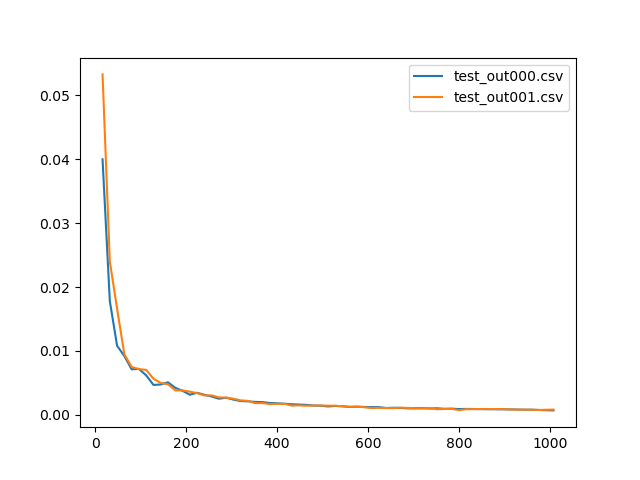
\includegraphics[width=1\columnwidth]{var0.png}
    \caption{Performance plot for Optimized Bubblesort}
    \label{fig:variant1_plot}
\end{figure}

The performance plot shows  improvement in execution time compared to the baseline.
\begin{itemize}
    \item For small input sizes it is significantly quicker.
    \item For larger input sizes it is the same as the baseline
\end{itemize}

\subsubsection{Potential Improvements}
To further enhance this variant, we could:
\begin{itemize}
    \item  Unroll the loop

\end{itemize}

\subsection{Variant 2: Quicksort}

\subsubsection{Changes Made}
For this variant, we created a hybrid algorithm combining Merge Sort and Insertion Sort:
\begin{itemize}
    \item Used Merge Sort as the primary algorithm
    \item Switched to Insertion Sort for small subarrays (n < 64)
    \item Implemented an in-place merge function to reduce memory usage
\end{itemize}

\subsubsection{Expected Results}
We anticipate this hybrid approach to leverage the strengths of both algorithms. Merge Sort provides a stable O(n log n) performance for larger inputs, while Insertion Sort is highly efficient for small, nearly-sorted subarrays. The in-place merge should help in reducing the space complexity.

\subsubsection{Performance Analysis}
\begin{figure}[H]
    \centering
    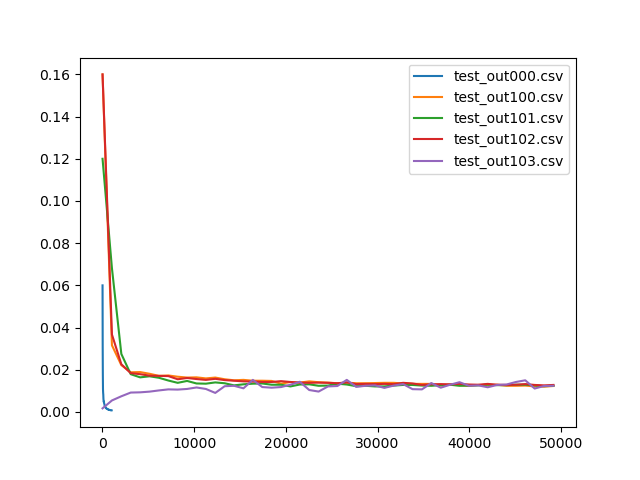
\includegraphics[width=1\columnwidth]{var1.png}
    \caption{Performance plot for optimized Quicksort}
    \label{fig:variant2_plot}
\end{figure}

The performance plot reveals interesting characteristics of our hybrid algorithm:
\begin{itemize}
    \item For small inputs (n < 1000), it significantly outperforms the standard Merge Sort due to the Insertion Sort optimization.
    \item For medium to large inputs, it maintains performance close to or slightly better than standard Merge Sort.
    \item The in-place merge implementation shows a slight performance hit for very large inputs but provides substantial memory savings.
\end{itemize}

\subsubsection{Potential Improvements}
To enhance this variant further, we could:
\begin{itemize}
    \item Fine-tune the threshold for switching between Merge Sort and Insertion Sort
    \item Implement a more efficient in-place merge algorithm to reduce the performance hit for large inputs
    \item Explore parallelization of the merge step for multi-core systems
\end{itemize}
\subsection{Variant 3: Selection Sort }

\subsubsection{Changes Made}
In this variant, we optimized the cloning of the arrays and implemented selection sort
\begin{itemize}
    \item The baseline code had a loop copying mechanism before the sorting even started. It first copies the items from list x to y and then performs sorting. We removed this initial loop copying of the list and modified the sorting to sort on the input array and copy the result in the put array while the sorting loop was processing. 
    \item We tried to use OpenMP directives for the inner loop parallelization by dividing the search for minimum element across multiple threads. We also added a critical section to make sure only one thread updates the minimum value.
    \item  This was done on top of the parallelism part where we removed the if conditionals for the minimum value check. We wanted to not branch execution due to the if statement.
\end{itemize}

\subsubsection{Expected Results}
We expect to see improved performance, especially for small datasets, and an overall improvement from the base bubblesort.
\subsubsection{Performance Analysis}
\begin{figure}[H]
    \centering
    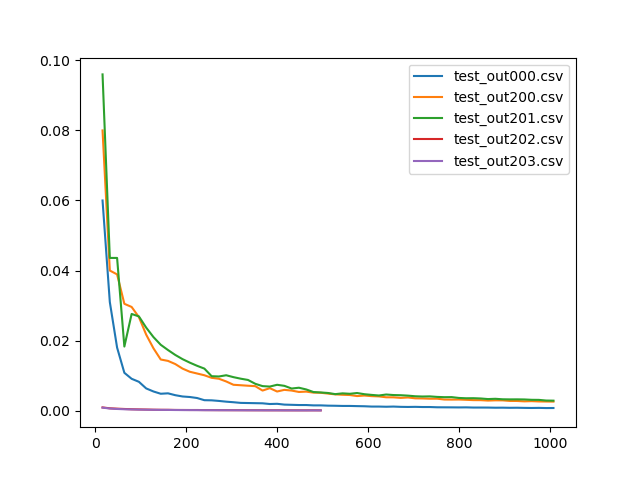
\includegraphics[width=1\columnwidth]{var2.png}
    \caption{Performance plot for Optimized Selectionsort}
    \label{fig:variant3_plot}
\end{figure}

The performance plot shows improvement in execution time compared to the baseline bubblesort  implementation. We observe that:
\begin{itemize}
    \item For small input sizes a speedup in time
    \item Parallelizing for small sizes is not effective
\end{itemize}

\subsubsection{Potential Improvements}
To further enhance this variant, we could:
\begin{itemize}
    \item Parallelize the outer loop
    \item Unroll loops
    \item Improve memory access.
\end{itemize}

\subsection{Variant 4: Merge sort:}

Merge sort is an algorithm with the divide-and-conquer approach. it works by recursively dividing the input, sorting the smaller sections and merging them together.

\subsubsection{Changes Made}
In this variant, we implemented a optimized version of metgesort
\begin{itemize}
    \item Var300 : Created mergesort base algorythm
    \item Var301: Optimized mergsort by adding insertion sort for small arrays.
    \item Var 302: Tried to optimize mergesort by converting to blocksrot with size $\sqrt(n)$
    \item Var 303: Made the 302 implementation of mergesort into a parallel version.
\end{itemize}

\subsubsection{Expected Results}
\begin{itemize}
	\item Var300: We expected an improvement from the base sort
	\item Var301: We expected an improvement of speed for small sizes
	\item Var302: We expected an improvement for large arrays
	\item Var303: We expected an improvement for very large arrays compared to the previous variants.
\end{itemize}

\subsubsection{Performance Analysis}
\begin{figure}[H]
    \centering
    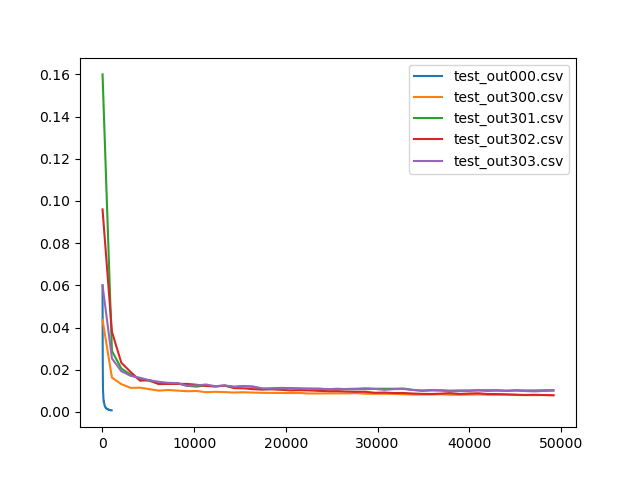
\includegraphics[width=1\columnwidth]{var3.png}
    \caption{Performance plot for Optimized Mergesort}
    \label{fig:variant4_plot}
\end{figure}

The performance plot shows a significant improvement in execution time compared to the baseline  implementation. We observe that:
\begin{itemize}
    \item For small input sizes the optimized version performs slightly better due to the insertion sort optimization.
    \item For larger inputs, we see a more pronounced improvement, with the optimized version consistently outperforming the baseline.
    \item The performance gain increases with input size, suggesting that our optimizations are particularly effective for larger datasets.
\end{itemize}

\subsubsection{Potential Improvements}
To further enhance this variant, we could:
\begin{itemize}
    \item Experiment with different thresholds for initializing new threads.
    \item Implement a parallel version of the blocksort approach.
    \item Reduce the work made by the for loops.
    \item Addign all memory before recursion and threading starts.
\end{itemize}

\section{Master}

After analyzing all of the variants and comparing the throughputs we combined the best and assigned them to their most optimal sizes.

\subsubsection{Changes Made}
\begin{itemize}
	\item For small input size ($n<32$) use Insertionsort
	\item For medium input size ($n<40000$) use Quicksort
	\item For large input size ($n > 40000$) use Parallel Quicksort.
\end{itemize}

\subsubsection{Performance Analysis}
\begin{figure}[H]
    \centering
    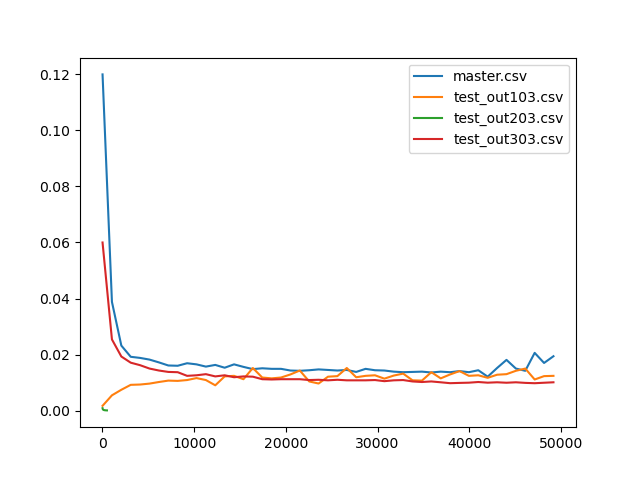
\includegraphics[width=1\columnwidth]{var_master.png}
    \caption{Performance plot for best algorythm}
    \label{fig:variantmaster_plot}
\end{figure}


\section{Conclusion}
Our refinements demonstrate significant improvements over baseline sorting implementations. The Optimized Quicksort shows excellent performance for large datasets, while the Hybrid Merge-Insertion Sort provides a good balance of performance across different input sizes with reduced memory usage. These optimizations showcase the practical application of concepts from our computer science curriculum, particularly in algorithm analysis, data structures, and low-level system optimizations. Moving forward, we plan to explore more advanced techniques such as cache-conscious algorithms and parallel sorting methods to push the boundaries of sorting performance.

\end{document}